%%%%%%%%%%%%%%%%%%%% book.tex %%%%%%%%%%%%%%%%%%%%%%%%%%%%%
%
% sample root file for the chapters of your "monograph"
%
% Use this file as a template for your own input.
%
%%%%%%%%%%%%%%%% Springer-Verlag %%%%%%%%%%%%%%%%%%%%%%%%%%


% RECOMMENDED %%%%%%%%%%%%%%%%%%%%%%%%%%%%%%%%%%%%%%%%%%%%%%%%%%%
\documentclass[pdftex,12pt, oneside, a4paper]{book}

% choose options for [] as required from the list
% in the Reference Guide, Sect. 2.2
%\usepackage[paperwidth=8.5in, paperheight=13in]{geometry}

\usepackage{makeidx}         % allows index generation
\usepackage{graphicx}        % standard LaTeX graphics tool
                             % when including figure files
\usepackage[bottom]{footmisc}% places footnotes at page bottom
\usepackage[english]{babel}
\usepackage{enumerate}
\usepackage{paralist}
\usepackage{float}
\usepackage{gensymb}  
\usepackage{listings}
\usepackage{color} 
\usepackage{array}

% make quote in italic
\newenvironment{italicquotes}
  {\begin{quote}\itshape}
  {\end{quote}}
% etc.
% see the list of further useful packages
% in the Reference Guide, Sects. 2.3, 3.1-3.3

% definisi warna untuk kode program
\definecolor{codegreen}{rgb}{0, 0.6, 0}
\definecolor{codegray}{rgb}{0.5, 0.5, 0.5}
\definecolor{codepurple}{rgb}{0.58, 0, 0.82}
\definecolor{backcolor}{rgb}{0.95, 0.95, 0.92}

% list code custom style
\lstdefinestyle{mystyle} {
  backgroundcolor=\color{backcolor}, 
  commentstyle=\color{codegreen},
  keywordstyle=\color{magenta}, 
  numberstyle=\tiny\color{codegray},
  stringstyle=\color{codepurple},
  basicstyle=\footnotesize,
  breakatwhitespace=false, breaklines=true, captionpos=b, keepspaces=true,
  numbers=left, numbersep=5pt, showspaces=false, showstringspaces=false,
  showtabs=false, tabsize=2
}

% mystyle for listing set
\lstset{style=mystyle}

\newcommand{\HRule}{\rule{\linewidth}{0.5mm}}

\makeindex             % used for the subject index
                       % please use the style svind.ist with
                       % your makeindex program


%%%%%%%%%%%%%%%%%%%%%%%%%%%%%%%%%%%%%%%%%%%%%%%%%%%%%%%%%%%%%%%%%%%%%

\begin{document}

%\author{Priyanto Tamami}
%\title{BUKU PETUNJUK OPERASIONAL SISTEM INFORMASI GEOGRAFIS UNTUK PBB-P2 DENGAN MAPINFO VERSI 8.0}
%\date{22 Desember 2015}
%\maketitle

\begin{titlepage}

\begin{center}
{\large BUKU PETUNJUK IMPLEMENTASI QUANTUM GEOGRAPHICAL INFORMATION SYSTEM (QGIS) UNTUK DASAR PEMETAAN PBB-P2}

\HRule\\[1cm]

PERIODE PENILAIAN TAHUN 2016\\[1cm]


\includegraphics[width=0.5\textwidth]{./resources/logo}\\[1cm]

Oleh :\\
Priyanto Tamami, S.Kom.\\
NIP 19840409 201001 1 025\\
Dinas Pendapatan dan Pengelolaan Keuangan\\
Pemerintah Kabupaten Brebes\\[1cm]

\vfill

Tim Penilai\\
Jabatan Fungsional Pranata Komputer\\
Badan Pusat Statistik\\
Brebes, 26 Mei 2016
\end{center}

\end{titlepage}

\frontmatter%%%%%%%%%%%%%%%%%%%%%%%%%%%%%%%%%%%%%%%%%%%%%%%%%%%%%%

%\include{dedic}
%\include{pref}

\begin{center}
{\huge \bfseries Lembar Pengesahan}\\[0.4cm]

\begin{tabular}{l c p{10cm}}
  Nama Kegiatan & : & Membuat Petunjuk Operasional Sistem Komputer \\
  Judul & : & BUKU PETUNJUK IMPLEMENTASI QUANTUM GEOGRAPHICAL INFORMATION SYSTEM (QGIS) UNTUK DASAR PEMETAAN PBB-P2 \\
\end{tabular}\\[2cm]

\begin{tabular}{c c}
  Disetujui oleh : & Disusun Oleh \\
  Kepala Seksi Pendataan, Penetapan, dan Keberatan & Pranata Komputer \\
  Pada tanggal 27 Mei 2016 & Selesai tanggal : 26 Mei 2016 \\
  & \\
  & \\
  & \\
  Fetiana Dwiningrum, SIP, M.Si. & Priyanto Tamami, S.Kom \\
  NIP 19880223 200701 2 001 & NIP 19840409 201001 1 025
\end{tabular}

\end{center} 

\tableofcontents
\listoffigures

\mainmatter%%%%%%%%%%%%%%%%%%%%%%%%%%%%%%%%%%%%%%%%%%%%%%%%%%%%%%%


\chapter{KONSEP DASAR SISTEM INFORMASI GEOGRAFIS (SIG)}

\begin{enumerate}[A.]
\item{Definisi}

Sistem Informasi Geografis (Geographic Information System / GIS) yang selanjutnya disebut SIG merupakan sistem informasi berbasis komputer yang digunakan untuk mengolah dan menyimpan data atau informasi geografis.

Secara umum pengertian SIG adalah sebagai berikut :
\begin{italicquotes}
Suatu komponen yang terdiri dari \textbf{perangkat keras, perangkat lunak, sumber daya manusia, dan data} yang bekerja bersama secara efektif untuk memasukkan, menyimpan, memperbaiki, memperbaharui, mengelola, memanipulasi, mengintegrasikan, menganalisa, dan menampilkan data dalam suatu informasi berbasis geografis.
\end{italicquotes}

Dalam pembahasan selanjutnya, SIG akan selalu diasosiasikan dengan sistem yang berbasis komputer, walaupun pada dasarnya SIG dapat dikerjakan secara manual, SIG yang berbasis komputer akan sangat membantu ketika data geografis merupakan data yang besar (dalam jumlah dan ukuran) dan terdiri dari banyak tema yang saling berkaitan.

SIG mempunyai kemampuan untuk menghubungkan berbagai data pada suatu titik tertentu di bumi, menggabungkannya, menganalisa, dan akhirnya memetakan hasilnya.

\item{Komponen SIG}
\end{enumerate}

\chapter{DATA SIG (Format dan Sumber Data)}


\chapter{INSTALASI QGIS}

Cara instalasi aplikasi QGIS berbeda antara menggunakan sistem operasi Windows dan sistem operasi Linux.

\begin{enumerate}[A.]

\item Instalasi QGIS di lingkungan Sistem Operasi Windows

Untuk sistem operasi Windows, perangkat lunak QGIS dapat di unduh secara gratis di \textit{website} resmi QuantumGIS dengan alamat http://qgis.org/ melalui berbagai macam \textit{web browser} seperti Firefox, Chrome, Opera, atau Internet Explorer. Tahapannya adalah sebagai berikut :

\begin{enumerate}[1.]

\item Pada kolom halaman di atas jendela \textit{browser}, masukan teks berikut dan tekan Enter : http://qgis.org/, sehingga muncul jendela pada gambar \ref{fig:qgishomepage} :

\begin{figure}
  \centering
  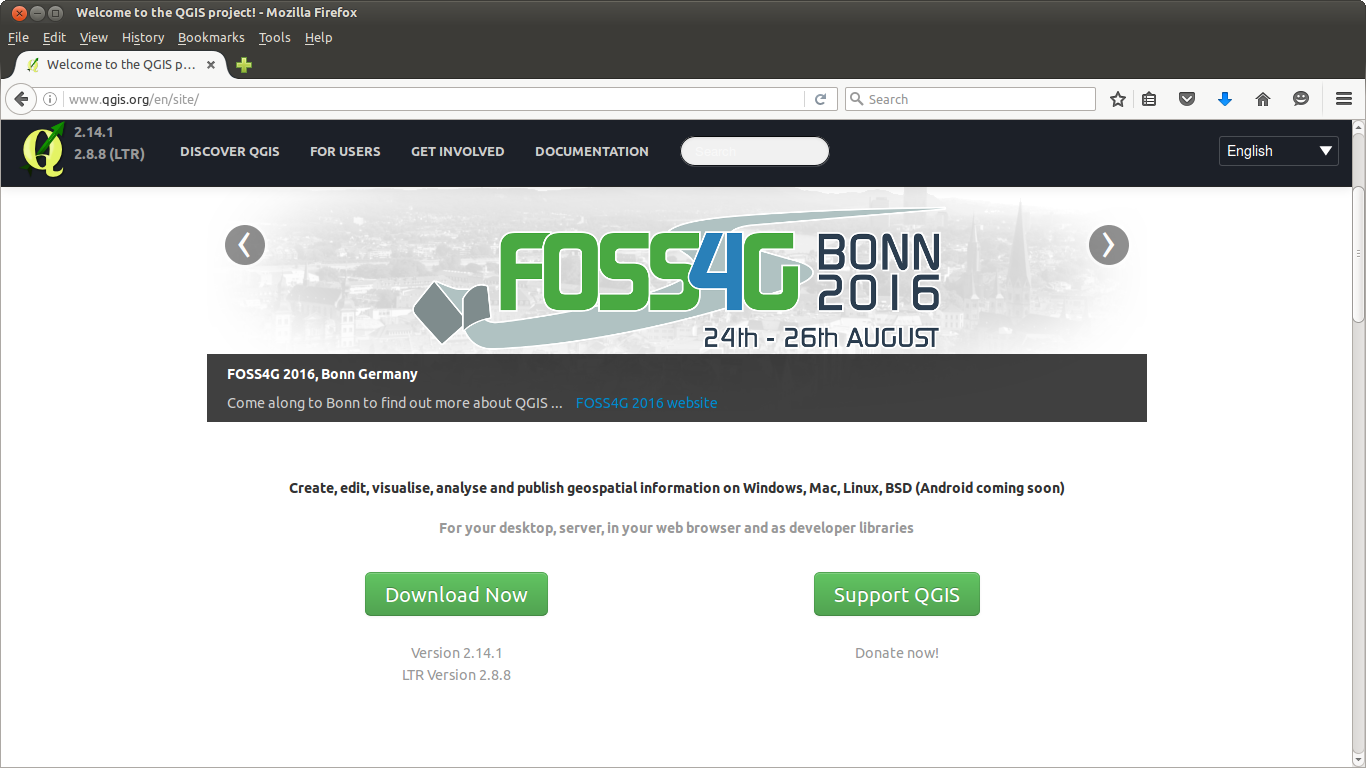
\includegraphics[width=1\textwidth]{./resources/001-homepage-qgis}
  \caption{Jendela \textit{website} QGIS}
  \label{fig:qgishomepage}
\end{figure}

\item Klik \verb|Download Now| pada halaman tersebut.

\item Pada jendela \textit{download} seperti ditampilkan dalam gambar \ref{fig:qgisversion} akan terdapat pilihan QGIS \textit{installer} berdasarkan sistem operasi perangkat yang anda gunakan. \textit{Expand} pilihan sistem operasi yang anda gunakan, lalu klik pada \textbf{Standalone Installer} (direkomendasikan untuk pengguna pemula).

\begin{figure}
  \centering
  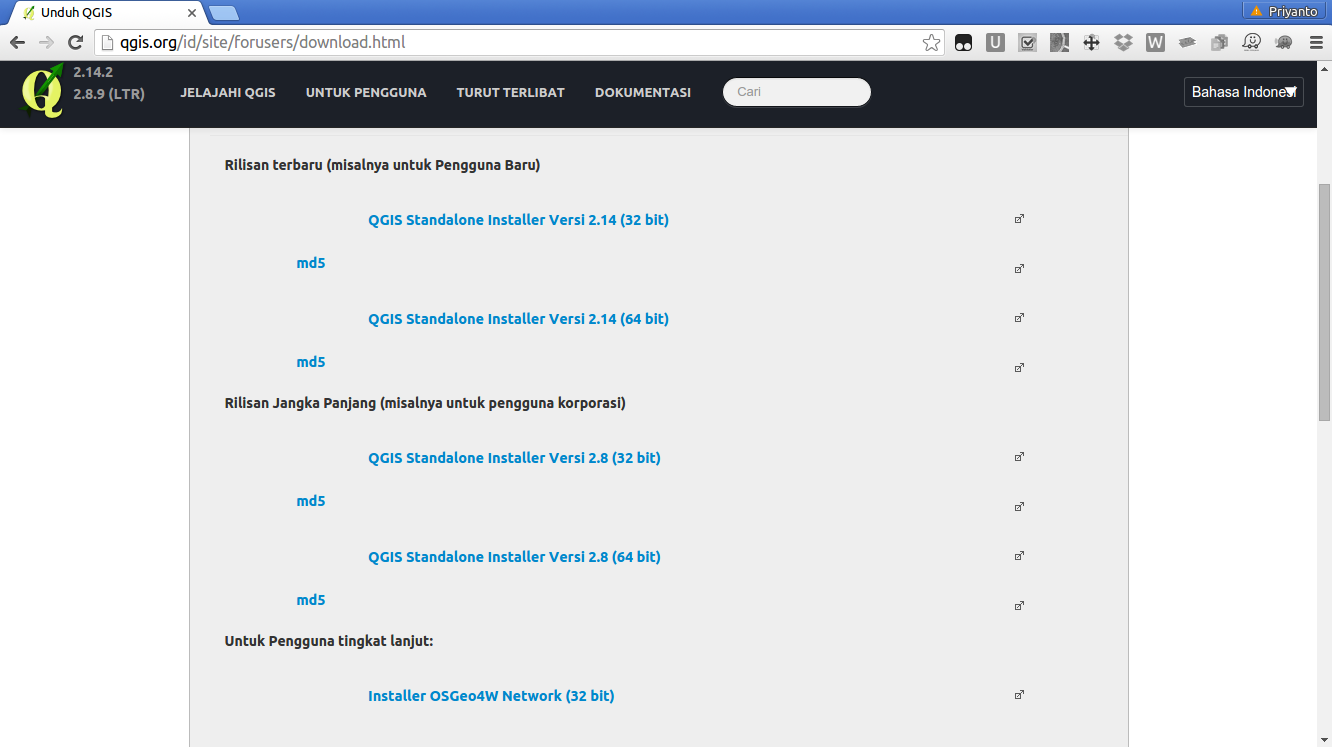
\includegraphics[width=1\textwidth]{./resources/002-pilihan-versi}
  \caption{Pilihan Versi QGIS}
  \label{fig:qgisversion}
\end{figure}

\item Apabila QGIS telah berhasil diunduh, cari \textit{file} instalasi pada direktori yang telah anda tentukan sebelumnya.

\item Klik dua kali pada \textit{file} instalasi tersebut untuk memulai penginstalan QGIS.

\end{enumerate}

\item Instalasi QGIS di lingkungan Sistem Operasi Linux (Debian/Ubuntu)

\end{enumerate} 
\chapter{PENGENALAN ANTARMUKA DAN MENAMBAHKAN DATA SIG PADA APLIKASI QGIS}

Pada Bab ini kita akan mengenal bagian-bagian dasar yang biasa digunakan untuk membuat peta menggunakan QGIS 2.14, menambahkan data, dan mengeksplor data menggunakan \textit{tools-tools} yang tersedia.

\begin{enumerate}[A.]

\item \textbf{Pengenalan Antarmuka QGIS 2.14 Essen}

Bagian-bagian dari antarmuka QGIS ini seperti terlihat pada gambar \ref{fig:bagianui}.

\begin{figure}
  \centering
  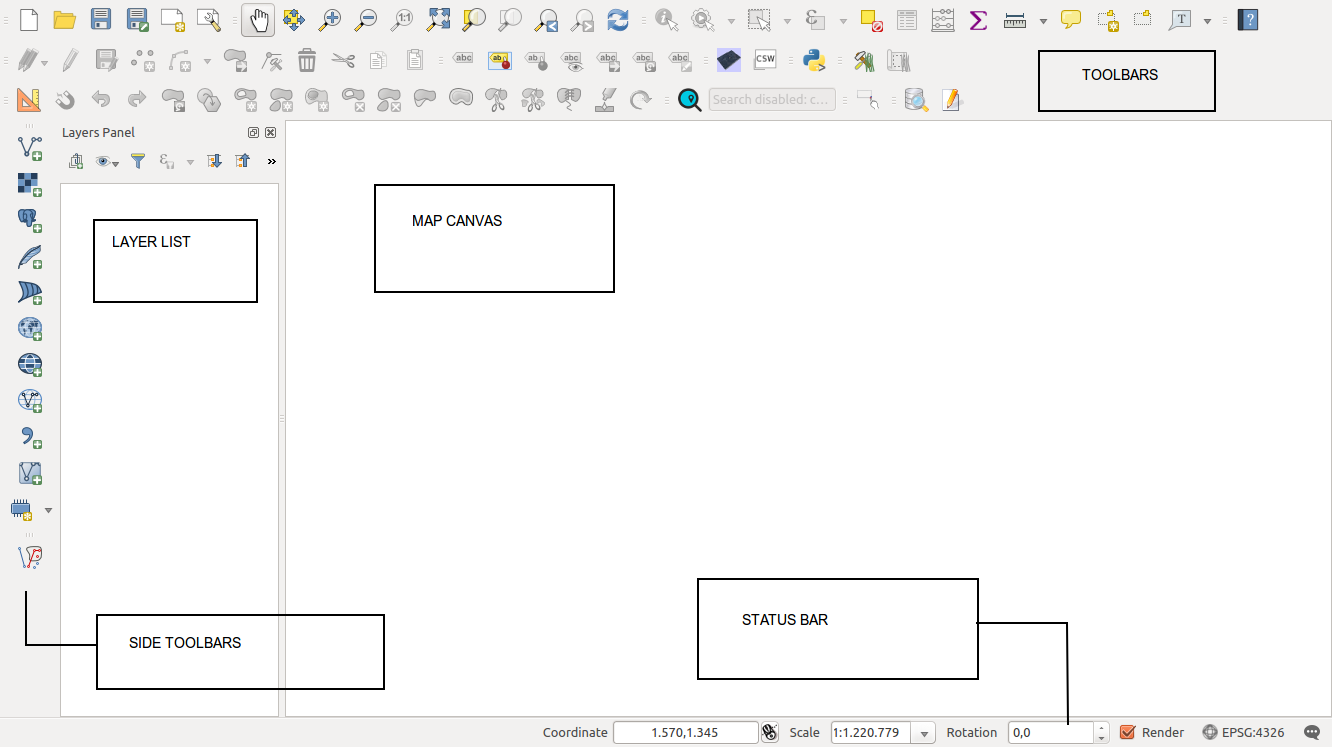
\includegraphics[width=1\textwidth]{./resources/004-bagian-qgis}
  \caption{Bagian Antarmuka QGIS}
  \label{fig:bagianui}
\end{figure}

\begin{itemize}

\item \textbf{Map Canvas}

Merupakan tempat menampilkan proyek / peta yang sedang dijalankan.

\item \textbf{Layer List}

Memuat daftar \textit{layer-layer} yang digunakan dalam proyek. Urutan \textit{layer} yang ditampilkan pada \textit{map canvas} berdasarkan urutan dari atas ke bawah pada \textit{layer list}-nya.

\item \textbf{Menu}

Bagian \textit{menu} ini tidak terlihat di gambar karena konfigurasi tampilan \textit{menu} menempel pada \textit{menu bar desktop}. \textit{Menu} ini berisi sekumpulan perintah teks untuk melakukan tugas-tugas tertentu.

\item \textbf{Toolbar dan Side Tooldbar}

Bagian ini berisi sekumpulan perintah berbasis tombol / ikon untuk melakukan tugas-tugas tertentu. \textit{Tools} dikelompokan dalam grup-grup \textit{toolbar} seperti \textit{File Toolbar}, \textit{Digitizing Toolbar}, \textit{Managed Layers Toolbar}, dan lainnya.

\item \textbf{Status Bar}

\textit{Status bar} memuat koordinat berdasarkan lokasi kursor / pointer, skala, dan sistem koordinat proyek pada \textit{map canvas}.

\end{itemize}

\item \textbf{Menambahkan Data}

Dalam QGIS dan aplikasi GIS pada umumnya, data vektor dalam format \textit{shapefile} dan data \textit{raster} yang akan ditambahkan untuk membuat sebuah \textit{project} (\texttt{*.qgis}) yang telah dibuat, melainkan hanya menyimpan \textit{style} dari data tersebut. Data tetap berada pada \textit{direktori} tempat menyimpan data, oleh karena itu satu \textit{dataset} dapat digunakan untuk berbagai \textit{project}. Berikut langkah-langkah yang dilakukan untuk menambahkan data sebagai \textit{layer} dalam QGIS.

\begin{enumerate}[1.]
  \item Klik \textit{tool} \texttt{Add Vector Layer} yang terlihat seperti pada gambar \ref{fig:addvectorlayer}.
  
\begin{figure}[H]
  \centering
  
\includegraphics[scale=1]{./resources/005-ikon-add-vektor-layer}
  \caption{Ikon \textit{Add Vector Layer}}
  \label{fig:addvectorlayer}
\end{figure}

  \item Sebuah kotak dialog tempat untuk memilih \textit{file} yang akan ditambahkan ke dalam proyek QGIS akan muncul seperti pada gambar \ref{fig:addvectorlayerwindow}
  
\begin{figure}[H]
  \centering
  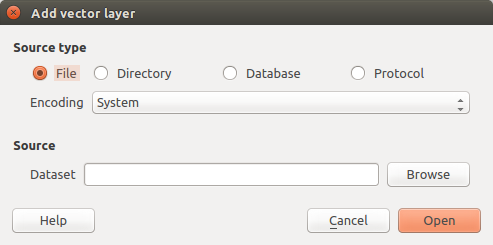
\includegraphics[scale=0.8]{./resources/006-add-vector-layer-window}
  \caption{Jendela \textit{Add Vector Layer}}
  \label{fig:addvectorlayerwindow}
\end{figure}

\end{enumerate}

\item \textbf{Mengeksplor Data}

\end{enumerate} 
\chapter{SISTEM REFERENSI KOORDINAT}

Pada kenyataannya bumi berbentuk seperti bola (3 dimensi) dengan permukaan yang tidak beraturan (Geoid). Untuk dapat menunjukkan lokasi suatu titik, garis, dan luasan di permukaan bumi diperlukan suatu bentuk matematis yang paling dekat dengan bentuk bumi yang sebenarnya, yaitu elipsoid.

Secara umum, terdapat 2 (dua) jenis koordinat yang sering digunakan, yaitu :

\begin{itemize}
  \item \textbf{Sistem Koordinat Geografis (Lintang - Bujur) / \textit{Geographic Coordinate System}}
  
    Pada sistem koordinat ini, bumi dibagi menjadi 360 (tiga ratus enam puluh) bagian, tiap bagian bernilai 1\degree, dan titik nol derajat adalah di Greenwich, Inggris. Disamping itu, garis khatulistiwa juga merupakan garis bujur 0\degree yang membagi dua wilayah, Di atas khatulistiwa sebagai wilayah utara dan di bawah khatulistiwa sebagai wilayah selatan. Dalam aplikasinya, wilayah selatan akan diberi simbol (-) minus, sedangkan (+) untuk wilayah utara. Sistem koordinat geografis seperti terlihat pada gambar \ref{fig:koordinatgeografis}
    
    \begin{figure}[H]
      \centering
      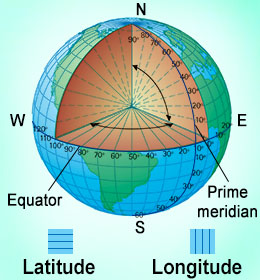
\includegraphics[scale=1]{./resources/015-koordinat-geografis}
      \caption{Koordinat Geografis}
      \label{fig:koordinatgeografis}
    \end{figure}
  
  \item \textbf{Sistem Koordinat Terproyeksi / \textit{Projected Coordinate System}}
  
    Apabila bentuk elipsoid disajikan dalam bidang datar. Maka diperlukan upaya transformasi dari bentuk 3D ke bentuk 2D melalui sistem proyeksi, seperti terlihat pada gambar \ref{fig:macamproyeksipeta}
    
    \begin{figure}[H]
      \centering
      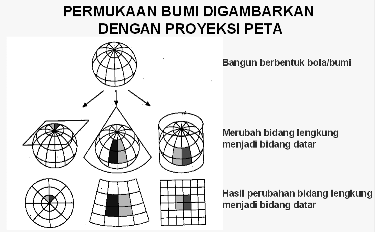
\includegraphics[scale=1]{./resources/016-macam-bidang-proyeksi-peta}
      \caption{Macam Bidang Proyeksi Peta}
      \label{fig:macamproyeksipeta}
    \end{figure}
    
    Tidak ada satu proyeksi yang bisa mempertahankan geometri asli. Semua proyeksi mempunyai distorsi geometri, namun masing-masing jenis proyeksi mempertahankan sifat aslinya, misalnya proyeksi yang mempertahankan luas permukaan (\textit{equivalen}), bentuk yang tetap (\textit{conform}), dan jarak yang tetap (\textit{ekuidistan}).
    
    Sistem proyeksi yang umum digunakan di Indonesia adalah \textbf{UTM (Universal Transverse Mercator)}. Untuk UTM, bumi kemudian dibagi ke dalam beberapa zona, antara 01 sampai dengan 60 dengan satuan meter. Pada sistem koordinat bumi akan dibagi menjadi dua bagian, di atas khatulistiwa sebagai bagian utara dengan simbol (N) serta di bagian selatan khatulistiwa di beri simbol (S).
    
    Sistem referensi koordinat yang paling cocok untuk seluruh wilayah di Indonesia adalah \textit{Geographic Coordinate System} yaitu WGS1984 (WGS84 / EPSG:4326). Sedangkan untuk wilayah satu provinsi atau lebih kecil sistem referensi koordinat yang paling cocok adalah \textbf{sistem koordinat terproyeksi} yaitu UTM WGS84. Contoh, untuk Jogja dan Jawa Tengah menggunakan UTM Zona 49S (WGS84 / UTM Zone 49S / EPSG:32749), seperti terlihat pada gambar \ref{fig:utmindonesia}.
    
    \begin{figure}[H]
      \centering
      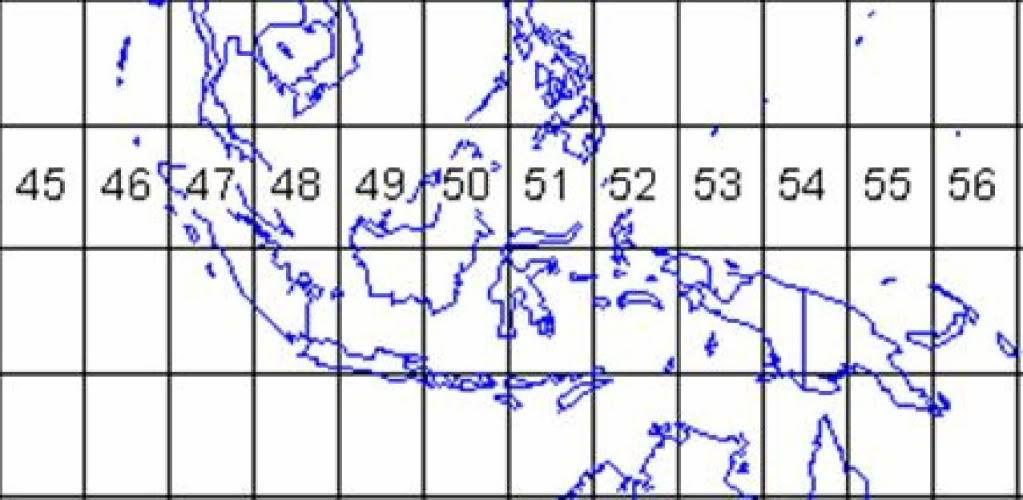
\includegraphics[width=1\textwidth]{./resources/017-utm-indonesia}
      \caption{Zona UTM di Indonesia}
      \label{fig:utmindonesia}
    \end{figure}
    
  \item \textbf{Sistem Referensi Koordinat / \textit{Coordinate Reference Systems (CRS)} di dalam QGIS}
  
    Dalam QGIS, sistem proyeksi Sistem Referensi Koordinat yang berbeda ditransformasikan secara otomatis menggunakan fitur \textit{on-the-fly} (OTF). Fitur ini memungkinkan pengguna untuk menampilkan \textit{layer} dengan CRS yang berbeda dan membuat \textit{layer-layer overlay} dengan benar. Namun terkadang kita memperoleh \textit{shapefile} yang tidak memiliki 

\end{itemize} 
\chapter{GEOREFERENSI DATA RASTER}

Jika kita mempunyai sebuah data raster yang berasal dari hasil \textit{scanning} peta, foto udara, dan citra satelit yang belum berisi informasi yang menunjukkan referensi spasial. Kemudian kita ingin melakukan digitasi berdasarkan data \textit{raster} tersebut. Maka yang diperlukan adalah membuat peta hasil \textit{scan} tersebut mempunyai sistem koordinat dengan melakukan koreksi geometrik yaitu proses \textit{georeference}. \textit{Georeference} merupakan proses transformasi koordinat pada data \textit{raster} dari koordinat \textit{scanner} ke koordinat \textit{real-world}.

Selain foto udara dan citra satelit, data \textit{raster} bisa diperoleh melalui hasil \textit{scanning} peta analog. Peta yang baik pasti memiliki informasi koordinat geografis yang ditunjukkan dengan \textit{Grid} pada peta tersebut.

Pada Bab ini, akan dipelajari bagaimana melakukan georeferensi terhadap data \textit{raster} hasil \textit{scanning} peta analog. Untuk memulai proses georeferensi tahapan-tahapan yang dilakukan adalah sebagai berikut :

\begin{enumerate}[1.]

  \item Pada jendela utama Quantum GIS, klik \texttt{Raster > Georeferencer > \- Georeferencer}, bila menu tersebut tidak muncul seperti gambar \ref{fig:georefmenunotexists}.
  
  \begin{figure}[H]
    \centering
    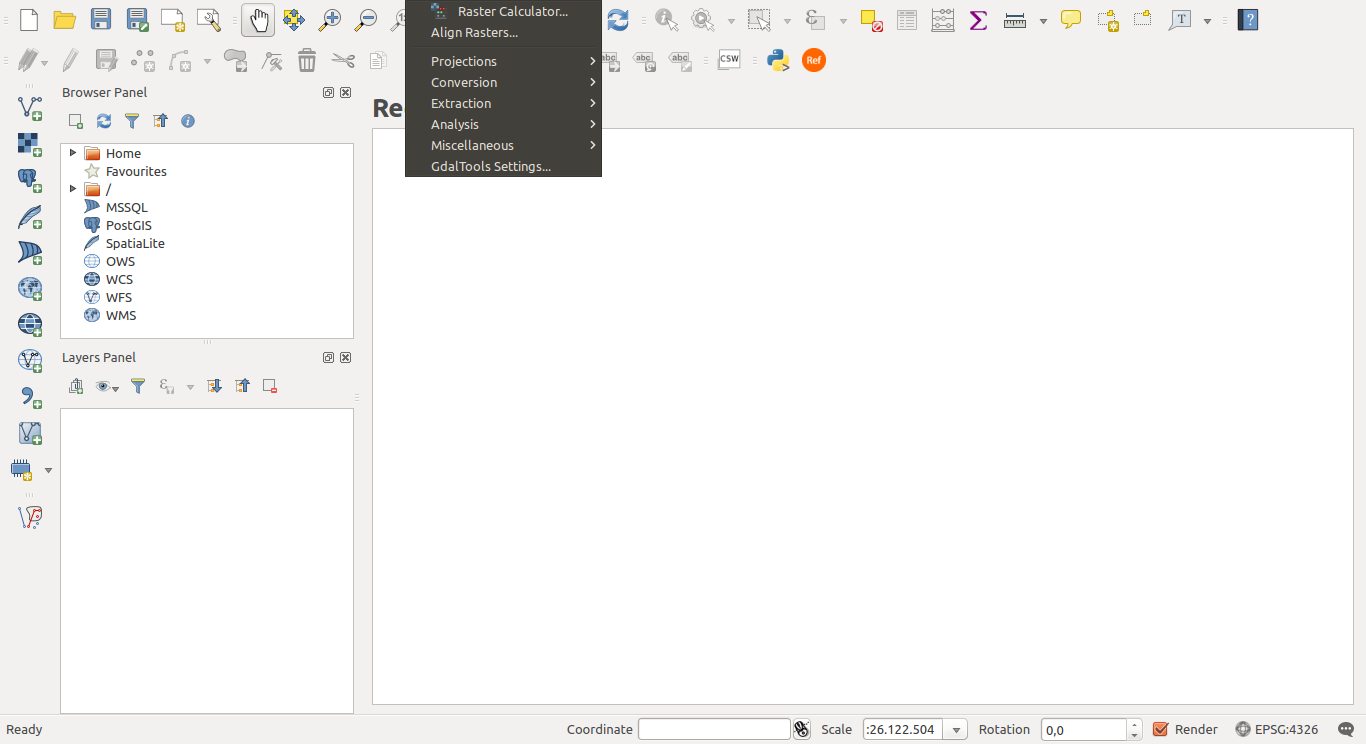
\includegraphics[width=1\textwidth]{./resources/018-menu-georeference-not-exists}
    \caption{Menu \textit{Georeference} tidak muncul}
    \label{fig:georefmenunotexists}
  \end{figure}
  
  Maka perlu memasangkan (\textit{install}) \textit{plugins} untuk \textit{georeferencer} terlebih dahulu dengan cara klik menu \verb|Plugins > Manage and Install Plugins...| sehingga muncul jendela pada gambar \ref{fig:pluginswin}.
  
  \begin{figure}[H]
    \centering
    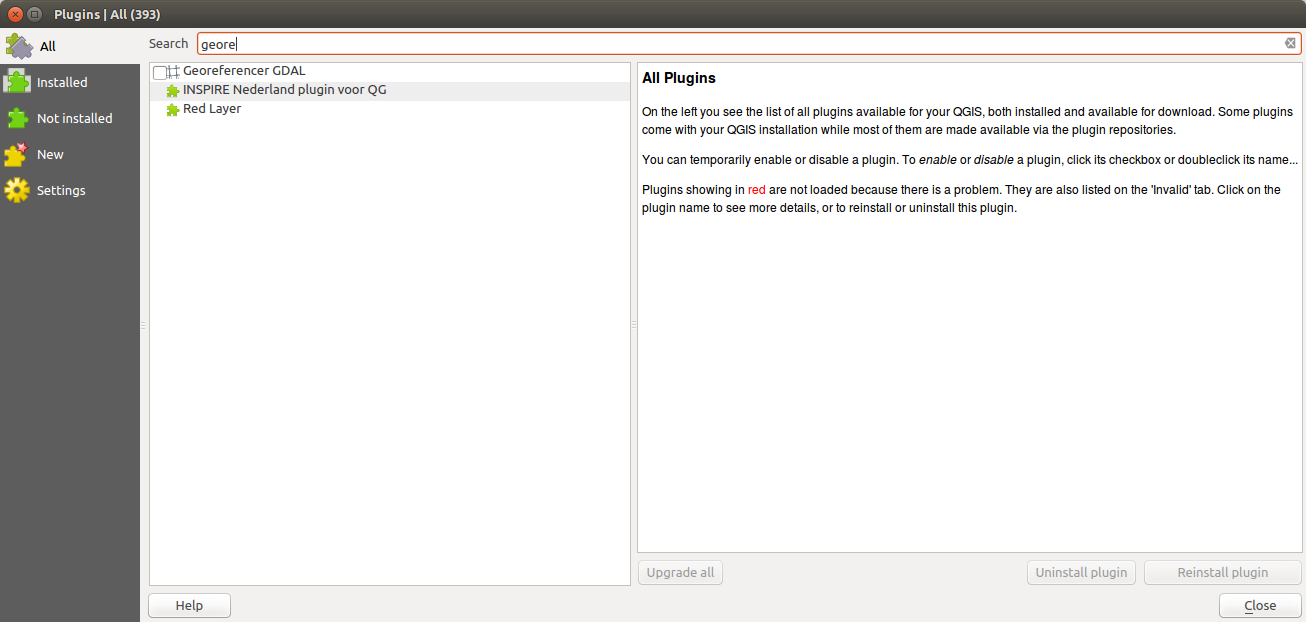
\includegraphics[width=1\textwidth]{./resources/020-pluginswin}
    \caption{Jendela \textit{Plugins}}
    \label{fig:pluginswin}
  \end{figure}
  
  sebelum jendela \textit{plugins} tersebut muncul, mungkin akan terlihat sebuah proses \textit{fetching repo} seperti pada gambar \ref{fig:fetchingrepo}.
  
  \begin{figure}[H]
    \centering
    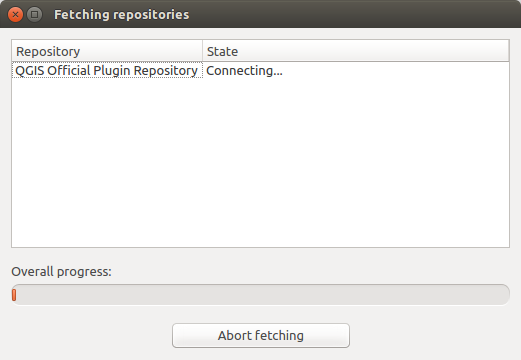
\includegraphics[width=1\textwidth]{./resources/019-fetching-repo}
    \caption{Jendela \textit{Fetching Repository}}
    \label{fig:fetchingrepo}
  \end{figure}
  
  Pada jendela \textit{plugins}, terdapat bagian \textit{search} untuk mempermudah mencari \textit{plugins} yang akan dipasang, ketikkan \verb|georeferencer| di kotak tersebut, lalu pilih tanda centang di sebelahnya. Bila belum terpasang, klik \verb|install plugin| di bagian jendela paling kanan bawah. Setelah selesai, maka akan muncul menu \verb|Georeferencer| pada menu \verb|Raster| seperti pada gambar \ref{fig:georefmenuexists}
  
  \begin{figure}[H]
    \centering
    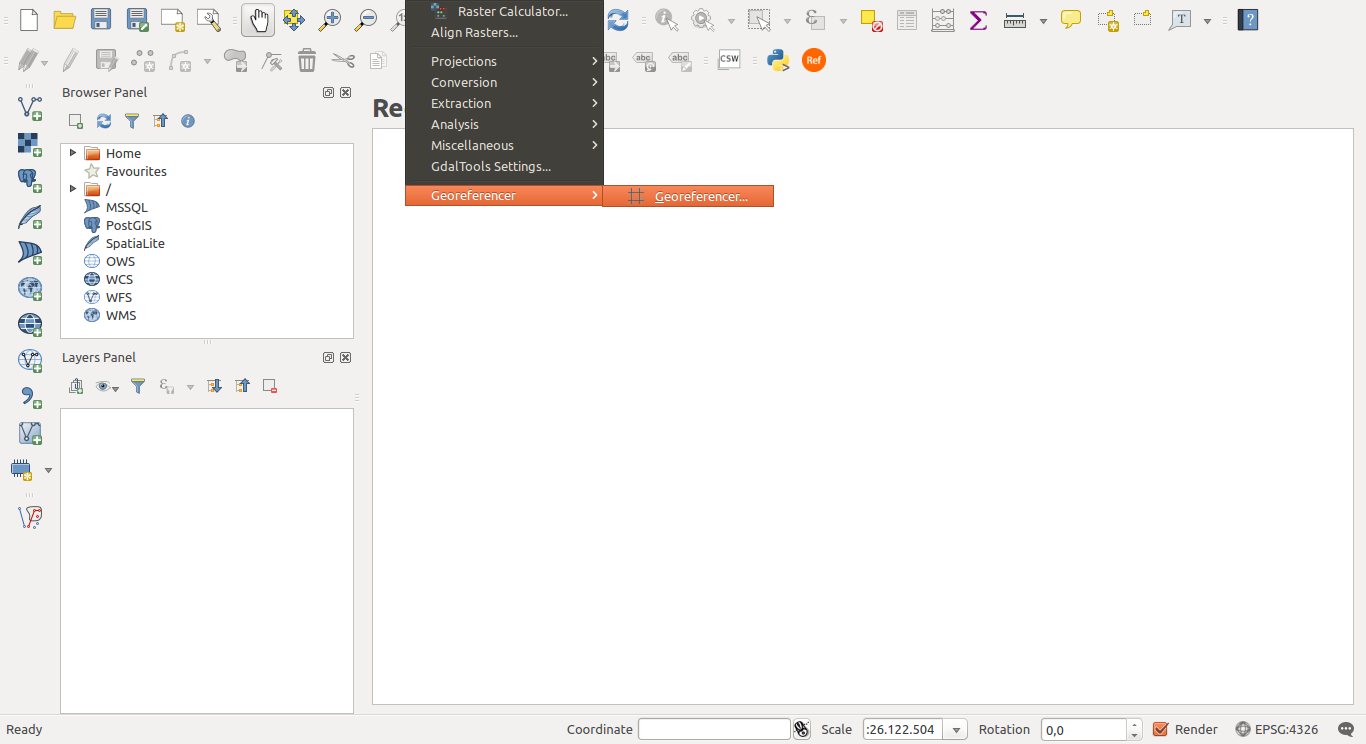
\includegraphics[width=1\textwidth]{./resources/021-georef-menu-exists}
    \caption{Menu \textit{Georeferencer} Muncul}
    \label{fig:georefmenuexists}
  \end{figure}
  
  Setelah memilih menu \verb|georeferencer| maka akan muncul jendela seperti pada gambar \ref{fig:georefwin}.
  
  \begin{figure}[H]
    \centering
    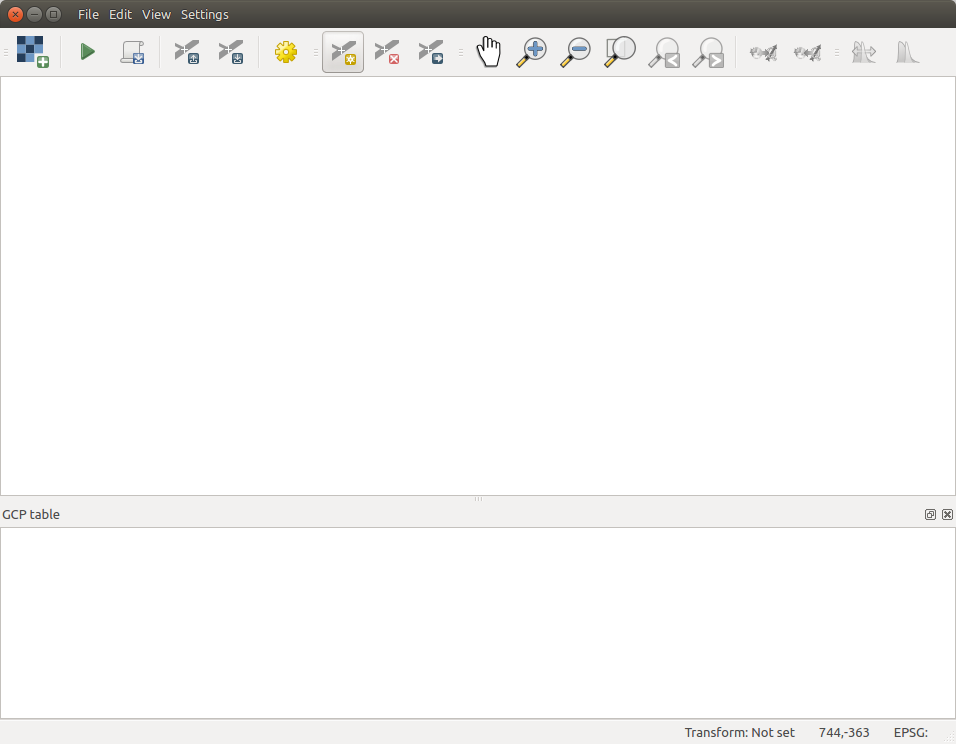
\includegraphics[width=1\textwidth]{./resources/022-georef-win}
    \caption{Jendela \textit{Georeferencer}}
    \label{fig:georefwin}
  \end{figure}
  
  \item Pada jendela \textit{georeferences}, klik \verb|File > Open Raster|. Kemudian pilih peta yang akan di georeferensi. Biasanya dalam bentuk JPG, atau GIF, atau bentuk format gambar yang lain yang didukung. Setelah membuka file \textit{raster} / gambar yang akan di georeferensikan, maka akan muncul gambar yang siap untuk diberikan koordinatnya seperti pada gambar \ref{fig:georeftif}
  
  \begin{figure}[H]
    \centering
    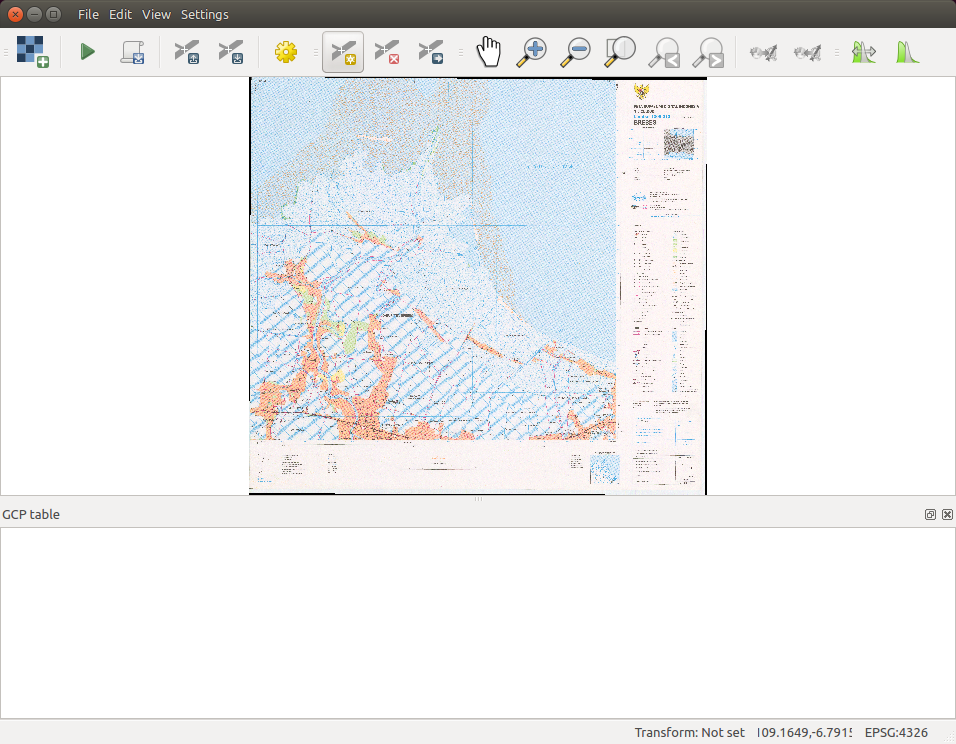
\includegraphics[width=1\textwidth]{./resources/023-georef-tif}
    \caption{\textit{File} TIF Yang Siap Untuk Digeoreferensikan}
    \label{fig:georeftif}
  \end{figure}
  
  Untuk memetakan 1 (satu) Kabupaten Brebes, sebetulnya lebih cocok menggunakan sistem koordinat terproyeksi seperti UTM, maka sumber data peta hasil \textit{scan} akan lebih memudahkan apabila terdapat informasi sebagaimana ditujukan pada gambar \ref{fig:refutm}.
  
  \begin{figure}[H]
    \centering
    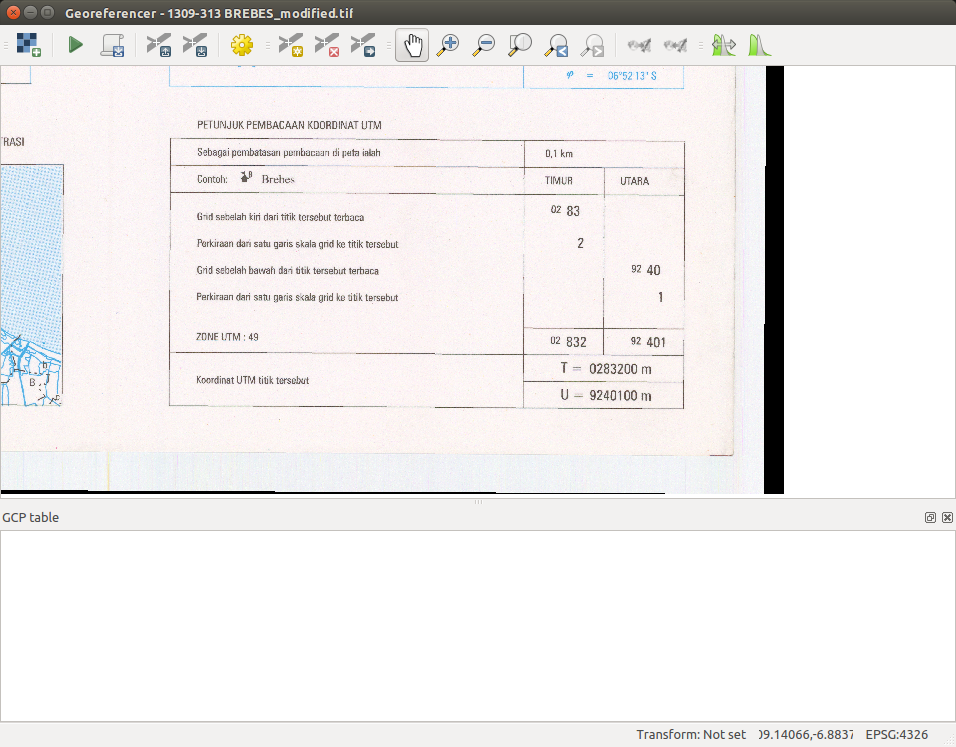
\includegraphics[width=1\textwidth]{./resources/024-utmpeta}
    \caption{Informasi Referensi UTM}
    \label{fig:refutm}
  \end{figure}
  
  Jika diperhatikan, maka peta hasil \textit{scan} tersebut masuk ke dalam zona 49. Karena informasi yang ditunjukkan oleh peta berada pada koordinat geografis S (\textit{South}) maka dapat dipastikan bahwa \textit{grid} peta tersebut berada pada zona 49S.
  
  Sebelum menentukan titik ikat, maka diperlukan proyeksi yang tepat terlebih dahulu dengan klik menu \verb|Settings > Transformation Settings...| atau klik ikon seperti gambar \ref{fig:transformationicon}
  
  \begin{figure}[H]
    \centering
    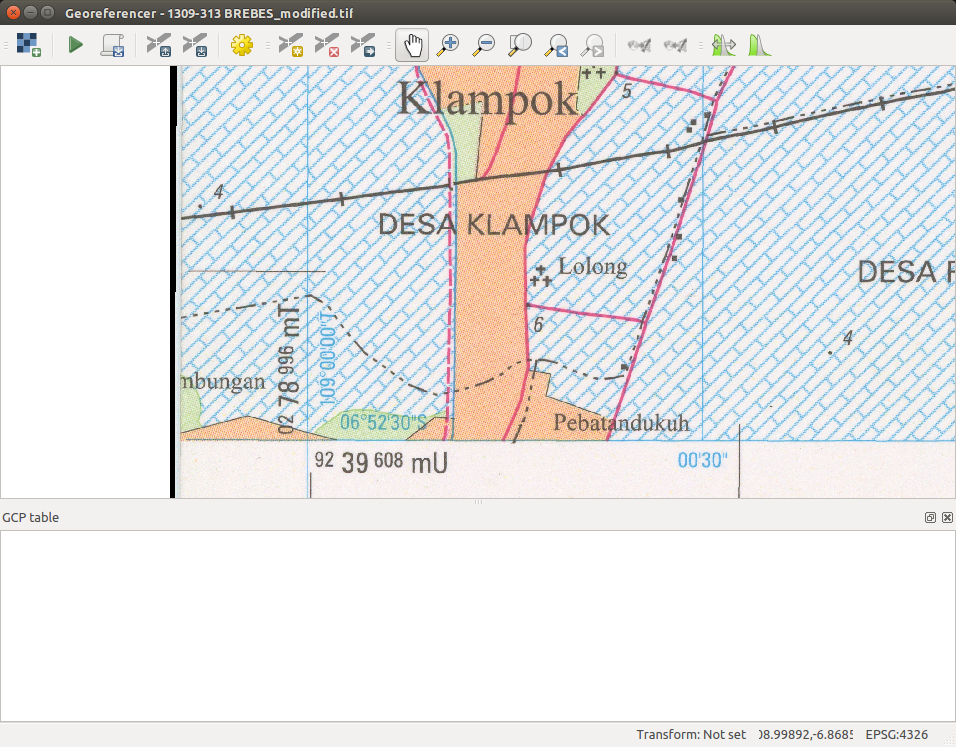
\includegraphics[scale=1]{./resources/025-icon-transformation}
    \caption{Ikon \textit{Transformation}}
    \label{fig:transformationicon}
  \end{figure}
  
  \item Setelah itu akan muncul jendela seperti pada gambar \ref{fig:transformationwin}.
  
  \begin{figure}[H]
    \centering
    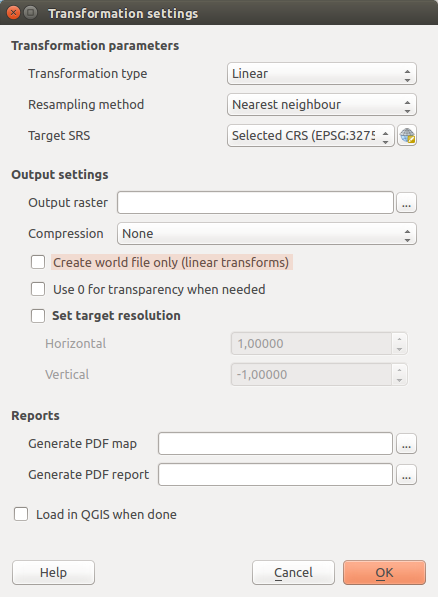
\includegraphics[width=1\textwidth]{./resources/026-transformation-win}
    \caption{Jendela Konfigurasi \textit{Transformation}}
    \label{fig:transformationwin}
  \end{figure}
  
  Yang perlu diperhatikan adalah pada bagian \verb|Target SRS|, pilihlah proyeksi yang tepat, yaitu \textbf{WGS 84 / UTM 49S} atau dengan kode yang lain adalah \textbf{EPSG:32749}. Sedangkan hasil proyeksinya dapat disimpan dalam 2 (dua) model, yang pertama akan berbentuk \textit{file} \textit{GeoTIFF} dengan ekstensi tif, dan yang kedua adalah \textit{file} tambahan berupa informasi koordinat dari \textit{raster} yang dimuat. Sehingga, untuk model yang pertama, kita tidak perlu melakukan georeferensi kembali saat memuat \textit{file GeoTIFF} ke QGIS, sedangkan untuk model yang kedua, kita tidak perlu melakukan georeferensi kembali untuk \textit{raster} yang sudah memiliki pasangan \textit{file} berupa informasi koordinat yang dihasilkan dari georeferensi ini.
  
  \item Selanjutnya membuat titik ikat atau \textit{Ground Control Point} (GCP) pada peta tersebut, maka pilih menu \verb|Edit > Add Point|, atau klik ikon seperti pada gambar \ref{fig:addpointicon}
  
  \begin{figure}[H]
    \centering
    
\includegraphics[scale=1]{./resources/027-add-point-icon}
    \caption{Ikon Tambah Titik Ikat}
    \label{fig:addpointicon}
  \end{figure}
  
  \item Apabila ingin menghapus titik ikat yang telah dibuat dapat menggunakan ikon \textit{Delete Point} seperti pada gambar \ref{fig:deletepointicon}.
  
  \begin{figure}[H]
    \centering
    
\includegraphics[scale=1]{./resources/028-delete-point-icon}
    \caption{Ikon Hapus Titik Ikat}
    \label{fig:deletepointicon}
  \end{figure}
  
  \item Sedangkan apabila ingin menggeser / memindahkan lokasi titik ikat, dapat menggunakan \textit{Move GCP Point} dengan melakukan klik pada ikon seperti pada gambar \ref{fig:movepointicon} dan arahkan pada titik ikat yang akan dipindahkan.
  
  \begin{figure}[H]
    \centering
    
\includegraphics[scale=1]{./resources/029-move-point-icon}
    \caption{Ikon Memindahkan Titik Ikat}
    \label{fig:movepointicon}
  \end{figure}
  
  \item Untuk memulai membuat titik ikat, pertama-tama \textit{Zoom} pada keempat pojok / sudut peta RBI untuk terlebih dahulu mengetahui lokasi dan nilai koordinat dari titik ikat yang akan digunakan.
  
  \item \textit{Zoom-in} di pojok kiri atas peta seperti pada gambar \ref{fig:rbismall}, kemudian buat titik di perpotongan \textit{grid} dengan tombol \textit{Add Point}, seperti yang ditunjukkan pada gambar \ref{fig:rbigrid}.
  
  \begin{figure}[H]
    \centering
    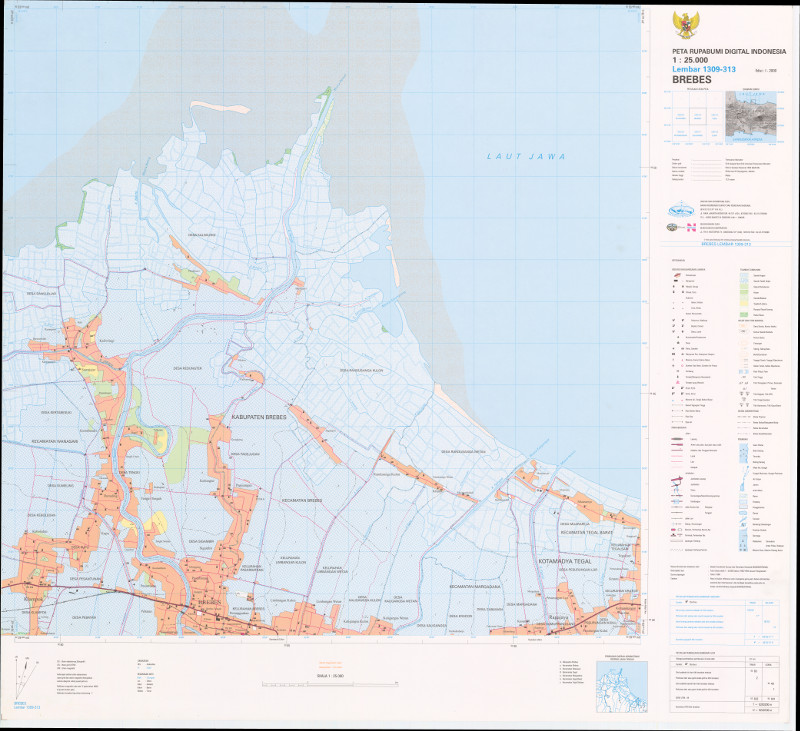
\includegraphics[width=1\textwidth]{./resources/030-rbi-brebes-resize-small}
    \caption{Peta Hasil \textit{Scan} RBI}
    \label{fig:rbismall}
  \end{figure}
  
  \begin{figure}[H]
    \centering
    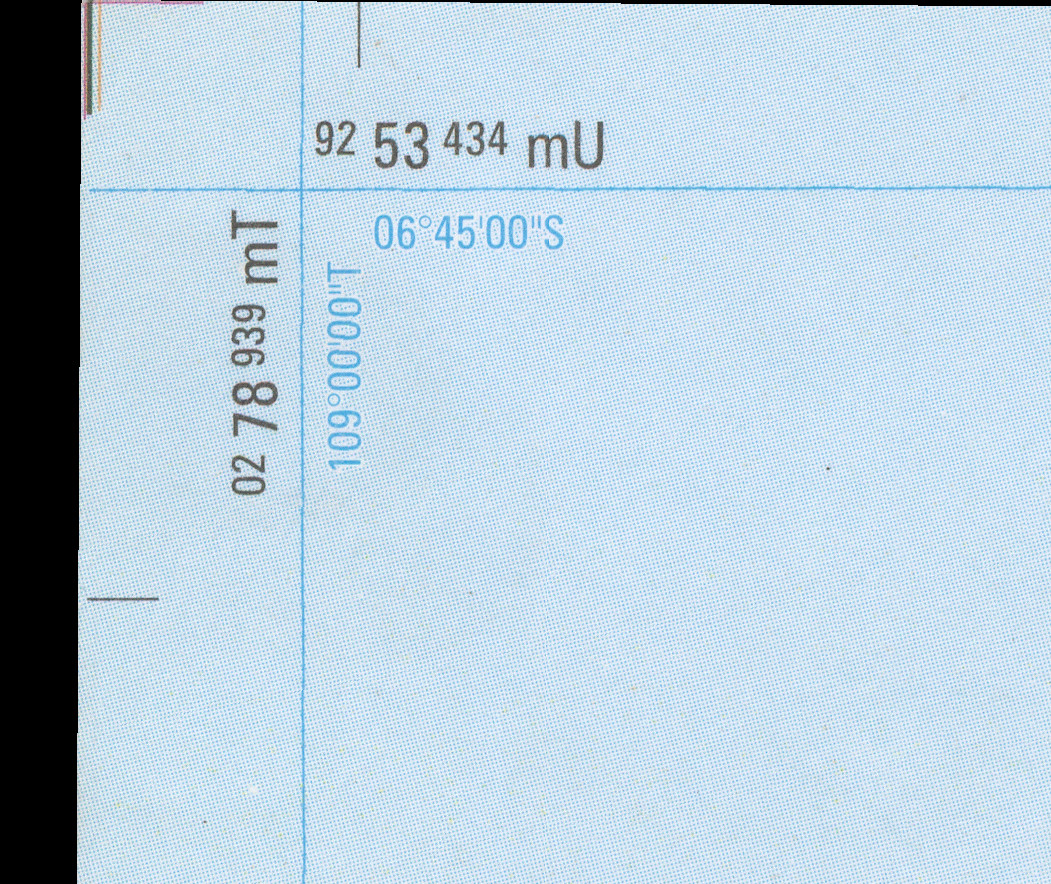
\includegraphics[width=1\textwidth]{./resources/031-rbi-brebes-crop-grid}
    \caption{Hasil \textit{Zoom-in} Pojok Kiri Atas Peta RBI}
    \label{fig:rbigrid}
  \end{figure}
  
  \item Setelah menambahkan titik ikat, maka otomatis akan keluar kotak dialog pengisian koordinat titik ikat tersebut seperti pada gambar \ref{fig:jendelatitikikat}. Isi koordinat sesuai yang ditunjuk oleh peta RBI, jika seperti contoh pada gambar \ref{fig:rbigrid}, artinya titik X akan berada pada 9253434, dan titik Y akan berada pada 0278939.
  
  \begin{figure}[H]
    \centering
    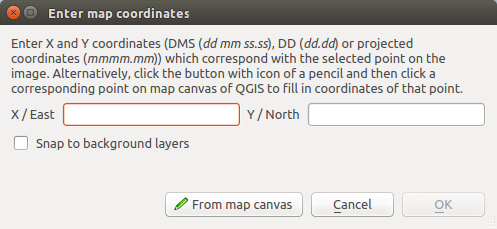
\includegraphics[width=1\textwidth]{./resources/032-jendela-georeferencer}
    \caption{Jendela \textit{Georeferencer}}
    \label{fig:jendelatitikikat}
  \end{figure}
  
  \item Lakukan hal yang sama untuk ketiga titik ikat lainnya sesuai dengan arah jarum jam.
  
  \item Tahap selanjutnya adalah menentukan pengaturan Transformasi untuk data \textit{raster} tersebut (Peta RBI), pilih menu \textit{Setting > Transformation Settings}, seperti yang ditunjukan pada gambar \ref{fig:transformationmenu}.
  
  \begin{figure}[H]
    \centering
    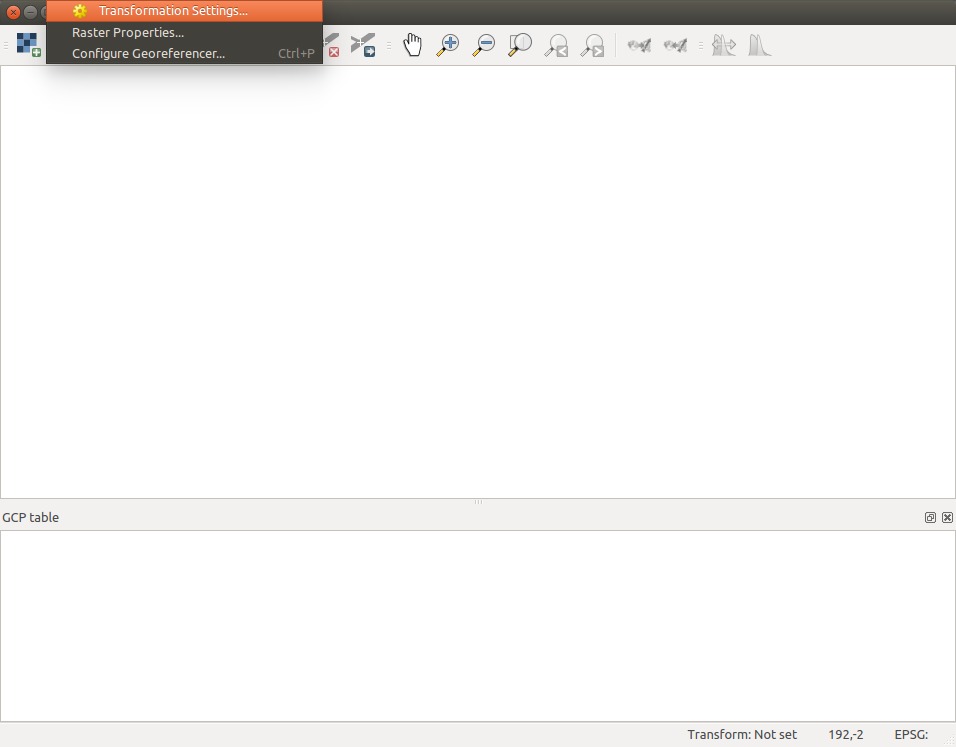
\includegraphics[width=1\textwidth]{./resources/033-menu-transformation}
    \caption{Menu \textit{Transformation}}
    \label{fig:transformationmenu}
  \end{figure}
  
  \item Setelah memilih menu \textit{Transformation}, akan muncul kotak dialog \textit{Transformation Setting}, tentukan tipe transformasi \textit{Linear}, dan metode \textit{Resampling} sesuai dengan yang diinginkan. Tentukan pula \textit{output raster}, dan pilih \verb|Create World File| sehingga nantinya dibuatkan \textit{file} referensi koordinat untuk gambar tersebut, dan jangan lupa untuk mengatur koordinat referensi yang digunakan, sesuaikan dengan zonanya.
  
  \item Setelah itu jalankan proses \textit{referencing} dengan menekan tombol \texttt{start \- Georeferencing} atau menekan ikon seperti pada gambar \ref{fig:startgeoref}
  
  \begin{figure}[H]
    \centering
    
\includegraphics[scale=1]{./resources/034-icon-start-georef}
    \caption{Ikon \textit{Georeferencing}}
    \label{fig:startgeoref}
  \end{figure}
  
  \item Tutup jendela \textit{Georeference}. Sekarang pada jendela utama QGIS, tampilkan peta \textit{raster} yang telah di \textit{georeference} dengan cara pilih \texttt{Layer > Add Raster Layer} atau klik tombol seperti pada gambar \ref{fig:addraster}
  
  \begin{figure}[H]
    \centering
    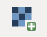
\includegraphics[scale=1]{./resources/035-icon-add-raster}
    \caption{Ikon \textit{Add Raster Layer}}
    \label{fig:addraster}
  \end{figure}
  
\end{enumerate} 
\chapter{MEMBUAT DATA SPASIAL (DIGITASI)}

Sebelumnya kita telah belajar bagaimana membuat peta sederhana dengan menampilkan Data Spasial yang telah disediakan. Tetapi, kita juga harus mempelajari bagaimana membuat Data Spasial yang baru, terutama jika kita tidak mempunyai Data Spasial tersebut. Misalkan, kita mempunyai sumber data \textit{raster} seperti citra satelit, foto udara, peta rupa bumi Indonesia, atau peta lainnya yang memiliki informasi koordinat, kita dapat membuat data spasialnya dengan melakukan digitasi terhadap data \textit{raster} tersebut.

\section{Pengertian Digitasi Peta}

Digitasi secara umum dapat didefinisikan sebagai proses konversi data analog ke dalam format digital. Objek-objek tertentu seperti jalan, rumah, sawah, dan lain-lain yang sebelumnya dalam format \textit{raster} maka menjadi objek-objek \textit{vektor}. Pada sebuah citra satelit resolusi tinggi dapat diubah kedalam format digital dengan proses digitasi.

\section{Metode Digitasi}

Proses digitasi secara umum dibagi dalam dua macam :

\begin{enumerate}[1.]

  \item Digitasi menggunakan \textit{digitizer} (zaman dulu, tetapi kini hampir tidak lagi), dalam proses digitasi ini memerlukan sebuah meja digitasi atau \textit{digitizer}.
  
  \item Digitasi \textit{on-screen} di layar monitor.
  
  Digitasi \textit{on-screen} paling sering dilakukan karena lebih mudah dilakukan, tidak memerlukan tambahan peralatan lainnya, dan lebih mudah untuk dikoreksi apabila terjadi kesalahan.
  
  Digitasi \textit{on-screen} biasanya dilakukan pada/dibantu oleh suatu \textit{base-layer} yang memiliki referensi spasial, misalnya citra satelit.

\end{enumerate}

\section{Membuat \textit{Shapefile}}

\begin{enumerate}[1.]

  \item Untuk membuat \textit{shapefile} baru pada QGIS, pilih menu \texttt{Layer > Create Layer > New Shapefile Layer} seperti pada gambar \ref{fig:menunewshape} atau dengan \textit{shortcut} \texttt{Ctrl + Shift + N}.
  
  \begin{figure}[H]
    \centering
    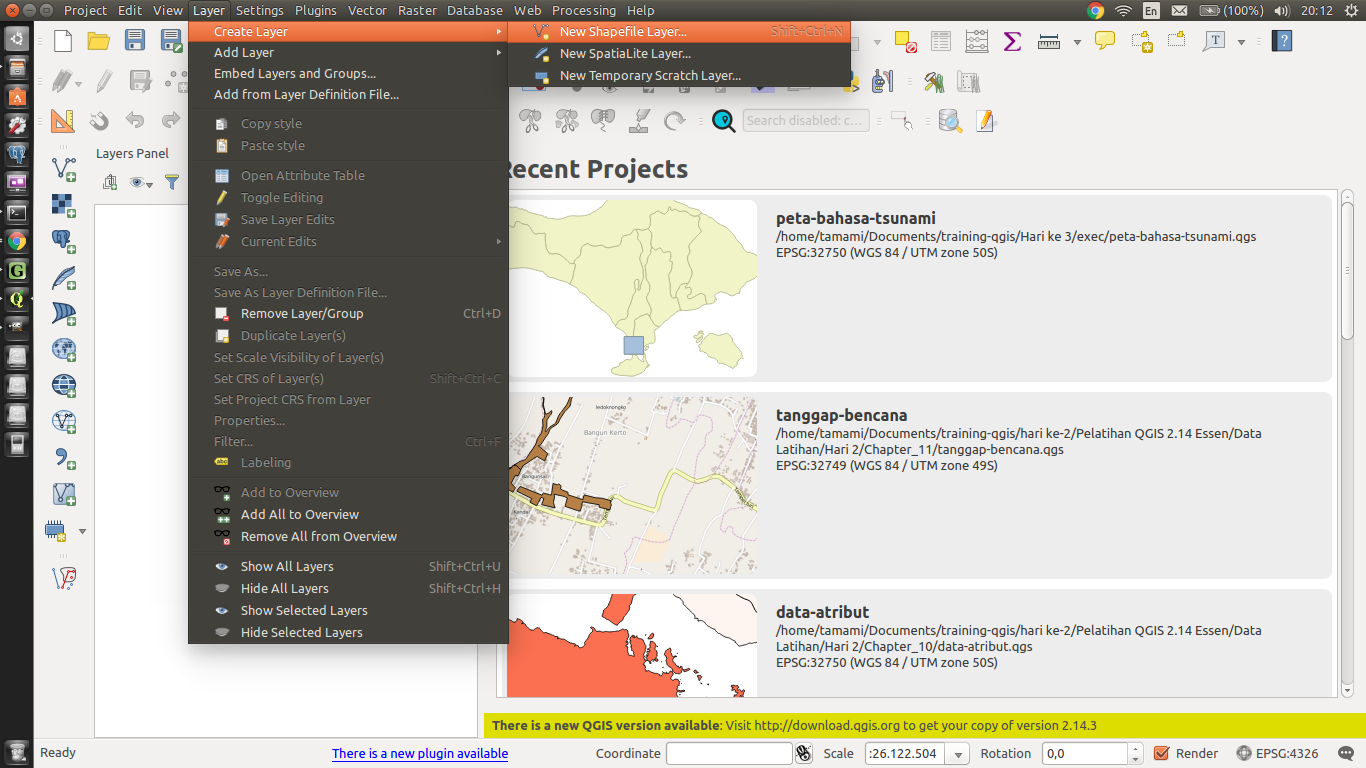
\includegraphics[width=1\textwidth]{./resources/036-menu-new-shape}
    \caption{Menu Menambahkan \textit{Layer Shapefile}}
    \label{fig:menunewshape}
  \end{figure}
  
  \item Kemudian akan muncul kotak dialog pembuatan \textit{layer} baru seperti gambar \ref{fig:newshapedialog}
  
  \begin{figure}[H]
    \centering
    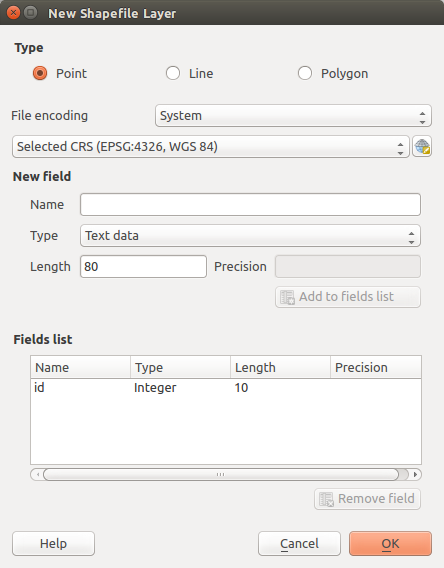
\includegraphics[width=1\textwidth]{./resources/037-new-shape-dialog}
    \caption{Jendela Pembuatan \textit{Layer Shapefile}}
    \label{fig:newshapedialog}
  \end{figure}
  
  Tipe \textbf{Point} adalah jenis \textit{layer} berupa titik yang digunakan untuk membuat \textit{Point of Interest}
  
  Tipe \textbf{Line} adalah jenis \textit{layer} berupa garis digunakan untuk membuat jalan, sungai, dan lainnya.
  
  Tipe \textbf{Polygon} adalah jenis \textit{layer} berupa area/luasan digunakan untuk membuat batas administrasi, \textit{landcover}, bangunan, dan lainnya.
  
  \item Tentukan sistem koordinatnya, di Indonesia sistem koordinat yang dipakai adalah WGS 1984. Apabila ingin menggunakan sistem koordinat UTM dengan zona UTM yang tentunya wilayah Kabupaten Brebes berada pada WGS84 UTM 49S (sebagai referensi tentang sistem koordinat yang digunakan, dapat melihat kembali bab tentang sistem koordinat).
  
  \item Membuat kolom pada data atribut.
  
  \begin{itemize}
  
    \item Buat nama kolom pada bagian \textit{Name}
    
    \item Tentukan tipe data yang ingin digunakan pada bagian \textit{Type}, keterangan untuk tiap tipe data adalah sebagai berikut :
    
    \begin{enumerate}[a.]
    
      \item \textbf{Tipe Data \textit{Text / String}} merupakan jenis data berupa teks, seluruh karakter termasuk \textit{alphanumeric} yang berjumlah maksimal 255 karakter.
      
      \item \textbf{Tipe Data \textit{Whole Number / Integer}} merupakan jenis data untuk bilangan bulat, seluruh angka termasuk positif dan negatif yang biasanya digunakan untuk menunjukkan nilai banyak (kuantitas) dari suatu tema, misalnya populasi penduduk.
      
      \item \textbf{Tipe Data \textit{Decimal Number / Real}} merupakan jenis data untuk bilangan pecahan yang biasa dituliskan dalam bentuk desimal dan memiliki \textit{range} yang spesifik. Dengan menggunakan tipe data ini, kita bisa 'menolak' sebuah nilai jika nilai tersebut diluar dari \textit{precision} dan \textit{scale} yang sudah ditentukan sebelumnya. Contoh : Kita menentukan \textit{precision} 4 (lebar \textit{field} hanya menerima maksimal 4 angka termasuk nilai \textit{decimal} tanpa memperhitungkan pemecahan angka tersebut, yaitu titik sebagai bentuk desimal) dan \textit{scale} 2 (maksimal 2 angka setelah pemecah angka tersebut, yaitu titik sebagai bentuk desimal), maka \textit{field} tersebut bisa menerima nilai 12,35 tetapi tidak dapat menerima nilai-nilai 1,235 dan 123,5. 
    
    \end{enumerate}
    
    \item Atur panjangnya karaketer yang dapat disimpan pada kolom \textit{width}.
    
    \item Khusus untuk tipe data \textit{Decimal Number} kita bisa mengatur panjangnya karakter sesudah koma yang dapat disimpan pada kolom \textit{Precision}
    
    \item Sebagai catatan saja bahwa nama \textit{field} terbatas hanya 10 karaketer saja dan hanya bisa menggunakan huruf, angka, \textit{hypens}, dan \textit{underscore}. Sepasang karakter dibolehkan tetapi tidak disarankan. Tidak bisa memberi nama \textit{field} menggunakan spasi atau spesial karakter lainnya, misalnya tanda tanya (?).
    
    \item Nama \textit{shapefile} boleh maksimal 10 karaketer (huruf, angka, underscore "\_").
  
  \end{itemize}
  
  \item Apabila sudah terisi semua, baik dari nama \textit{field}, tipe data, dan panjangnya data, kemudian klik \texttt{Add to fields list} untuk menambahkan daftar atribut yang akan dipasangkan pada \textit{shapefile} yang dibuat.
  
  \item Jika sudah selesai, tekan tombol \verb|OK| sehingga muncul jendela untuk menyimpan \textit{file} untuk \textit{layer shapefile} ini.

\end{enumerate}

Penentuan nama \textit{file} dan atributnya sudah dijadikan standar dengan penjelasan sebagai berikut :

\begin{itemize}

  \item \textit{Layer} Tanah / Bidang
  
  \textit{Layer} ini berisi tanah / bidang objek pajak dalam satu Desa / Kelurahan, dimana penamaan \textit{file} untuk layer tanah / bidang mengikuti format \texttt{3329KKKLLL}, dimana polanya adalah sebagai berikut :
  
  \begin{itemize}
    \item \texttt{33} adalah 2 (dua) digit kode Propinsi Jawa Tengah, sehingga sifatnya mutlak.
    \item \texttt{29} adalah 2 (dua) digit kode Kabupaten Brebes, sehingga sifatnya mutlak.
    \item \texttt{KKK} adalah 3 (tiga) digit kode Kecamatan di Kabupaten Brebes yang dapat dilihat pada basis data SISMIOP sebagai referensi.
    \item \texttt{LLL} adalah 3 (tiga) digit kode Kelurahan/Desa di Kabupaten Brebes yang dapat dilihat pada basis data SISMIOP sebagai referensi.
  \end{itemize}
  
  \textit{Layer} ini bertipe \textbf{poligon}, dengan \textit{fill patter} \textbf{none}, \textit{border style} \textbf{garis penuh}, \textit{color} \textbf{black} dan \textit{width} \textbf{0,17mm}. 
  
  Struktur data yang ada pada \textit{layer} tanah / bidang ini adalah seperti pada tabel berikut :
  
  \begin{table}[H]
    \centering
    \begin{tabular}{| c | c | c | p{7cm} |}
      \hline
      Field & Tipe & Index & Keterangan \\
      \hline \hline
      \textbf{d\_nop} & character(18) & index1 & NOP setiap bidang tanah \\
      \hline
      \textbf{d\_luas} & decimal(10,2) & & luas bidang tanah dengan menggunakan update kolom terhadap \textit{field} d\_luas dengan \textit{field calculator} \\
      \hline
    \end{tabular}
  \end{table}
  
  \item \textit{Layer} Bangunan
  
  \textit{Layer} ini berisi gambar denah bangunan dalam satu Desa/Kelurahan, dimana penamaan \textit{file} mengikuti aturan \texttt{3329KKKLLLbg}, dimana polanya adalah sebagai berikut :
  
  \begin{itemize}
    \item \texttt{33} adalah 2 (dua) digit kode Propinsi Jawa Tengah, sifatnya mutlak.
    \item \texttt{29} adalah 2 (dua) digit kode Kabupaten Brebes, sifatnya mutlak.
    \item \texttt{KKK} adalah 3 (tiga) digit kode Kecamatan yang dapat dilihat pada basis data SISMIOP sebagai referensi.
    \item \texttt{LLL} adalah 3 (tiga) digit kode Kelurahan yang dapat dilihat pada basis data SISMIOP sebagai referensi.
  \end{itemize}
  
  \textit{Layer} ini memiliki ciri fisik lain yaitu bertipe \textbf{poligon}, dengan \textit{fill pattern} seperti \textbf{MapInfo no. 5}, \textit{foreground} seperti \textbf{MapInfo no. 7}, \textit{background} \textbf{none}, \textit{border style} \textbf{garis putus}, \textit{line style} seperti \textbf{MapInfo no. 5}, \textit{color} \textbf{hijau}, dan \textit{width} \textbf{0,17mm}.
  
  Struktur basis data untuk \textit{layer} bangunan ini adalah sebagai berikut :
  
  \begin{table}[H]
    \centering
    \begin{tabular}{| c | c | c | p{7cm} |}
      \hline
      Field & Tipe & Index & Keterangan \\
      \hline\hline
      \textbf{d\_nop} & character(21) & index1 & NOP ditambah nomor bangunan untuk tiap bangunannya \\
      \hline
    \end{tabular}
  \end{table}
  
  \item \textit{Layer} Jalan
  
  \textit{Layer} jalan ini berisi gambar jalan dalam satu Desa/Kelurahan, dimana penamaan \textit{file} untuk \textit{layer} ini mengikuti aturan \texttt{3329KKKLLLjl}, dengan keterangan sebagai berikut :
  
  \begin{itemize}
    \item \texttt{33} adalah 2 (dua) digit kode Propinsi Jawa Tengah.
    \item \texttt{29} adalah 2 (dua) digit kode Kabupaten Brebes.
    \item \texttt{KKK} adalah 3 (tiga) digit kode Kecamatan yang dapat dilihat pada basis data SISMIOP sebagai referensi.
    \item \texttt{LLL} adalah 3 (tiga) digit kode Kelurahan yang dapat dilihat pada basis data SISMIOP sebagai referensi.
  \end{itemize}
  
  \textit{Layer} ini memiliki ciri fisik yaitu bertipe \textbf{Polyline}, \textit{style} \textbf{garis penuh}, \textit{color} \textbf{red}, \textit{width} \textbf{0,17mm}.
  
  Struktur basis data untuk \textit{layer} jalan ini adalah sebagai berikut :
  
  \begin{table}[H]
    \centering
    \begin{tabular}{| c | c | c | p{7cm} |}
      \hline
      Field & Tipe & Index & Keterangan \\
      \hline\hline
      \textbf{d\_nm\_jln} & character(30) & & Nama Jalan \\
      \hline
      \textbf{d\_lbr\_jln} & Integer & & Lebar jalan (rata-rata lebar pada jalan tersebut) \\
      \hline
    \end{tabular}
  \end{table}
  
  \item \textit{Layer} Sungai
  
  \textit{Layer} ini berisi gambar sungai dalam satu Desa/Kelurahan, dimana penamaan \textit{file} untuk \textit{layer} ini mengikuti aturan \texttt{3329KKKLLLsg}, dengan keterangan berikut :
  
  \begin{itemize}
    \item \texttt{33} adalah 2 (dua) digit kode Propinsi Jawa Tengah.
    \item \texttt{29} adalah 2 (dua) digit kode Kabupaten Brebes
    \item \texttt{KKK} adalah 3 (tiga) digit kode Kecamatan yang dapat dilihat pada basis data SISMIOP sebagai referensi
    \item \texttt{LLL} adalah 3 (tiga) digit kode Kelurahan yang dapat dilihat pada basis data SISMIOP sebagai referensi.
  \end{itemize}
  
  \textit{Layer} ini memiliki ciri fisik bertipe \textbf{polyline}, dengan \textit{style} \textbf{garis penuh}, \textit{color} \textbf{blue}, dan \textit{width} \textbf{0,17mm}.
  
  Struktur basis data untuk \textit{layer} sungai ini adalah sebagai berikut :
  
  \begin{table}[H]
    \centering
    \begin{tabular}{| c | c | c | p{7cm} |}
      \hline
      Field & Tipe & Index & Keterangan \\
      \hline\hline
      \textbf{d\_nm\_sng} & character(30) & & Nama Sungai \\
      \hline
      \textbf{d\_lbr\_sng} & integer & & Lebar sungai (rata-rata lebar pada sungai tersebut) \\
      \hline
    \end{tabular}
  \end{table}
  
  \item \textit{Layer} Teks
  
  \textit{Layer} ini berisi keterangan teks dalam satu Desa/Kelurahan, penamaan \textit{file} untuk \textit{layer} ini mengikuti aturan \texttt{3329KKKLLLtx}, dengan keterangan sebagai berikut :
  
  \begin{itemize}
    \item \texttt{33} adalah 2 (dua) digit kode Propinsi Jawa Tengah
    \item \texttt{29} adalah 2 (dua) digit kode Kabupaten Brebes
    \item \texttt{KKK} adalah 3 (tiga) digit kode Kecamatan yang dapat dilihat pada basis data SISMIOP
    \item \texttt{LLL} adalah 3 (tiga) digit kode Kelurahan yang dapat dilihat pada basis data SISMIOP.
  \end{itemize}
  
  Struktur basis data untuk \textit{layer} teks ini adalah sebagai berikut :
  
  \begin{table}[H]
    \centering
    \begin{tabular}{| c | c | c | p{7cm} |}
      \hline
      Field & Tipe & Index & Keterangan \\
      \hline\hline
      \textbf{d\_text} & character(30) & & Sebagai penjelas / keterangan pada bidang cetak peta. \\
      \hline
    \end{tabular}
  \end{table}
  
  Kolom \texttt{d\_text} dapat berisi :
  
  \begin{itemize}
    \item Teks mengenai keseluruhan nama utilitas jalan, sungai, informasi nama wilayah yang bersebelahan, informasi lokasi penting, dan sebagainya, yang tidak termasuk \textit{layer-layer} lain berwarna hitam dengan tipe huruf \textit{italic} berukuran sesuai dengan gambar.
    \item Batas tepi jalan diperkeras berwarna merah ukuran garis paling tipis
    \item Batas tepi jalan tidak diperkeras berwarna coklat kekuningan berukuran garis paling tipis
    \item Batas tepi jalan TOL berwarna merah berukuran garis tipis nomor 2 (di MapInfo)
    \item Batas tepi sungai berwarna biru berukuran garis tipis nomor 2 (di MapInfo).
    \item Utilitas yang disertai dengan simbolnya.
  \end{itemize}
  
  \item \textit{Layer} Batas Blok
  
  \textit{Layer} ini menggambarkan batas blok dalam suatu Desa/Kelurahan, penamaan \textit{file} mengikuti aturan \texttt{3329KKKLLLbl} dengan keterangan sebagai berikut :
  
  \begin{itemize}
    \item \texttt{33} adalah 2 (dua) digit kode Propinsi Jawa Tengah
    \item \texttt{29} adalah 2 (dua) digit kode Kabupaten Brebes
    \item \texttt{KKK} adalah 3 (tiga) digit kode Kecamatan yang dapat dilihat pada basis data SISMIOP
    \item \texttt{LLL} adalah 3 (tiga) digit kode Kelurahan yang dapat dilihat pada basis data SISMIOP.
  \end{itemize}
  
  Ciri fisik dari \textit{layer} batas blok ini adalah bertipe \textbf{polygon}, \textit{fill pattern} \textbf{none}, \textit{border style} \textbf{garis putus dan titik}, \textit{line style} \textbf{setara MapInfo nomor 13}, \textit{color} \textbf{blue}, \textit{width} \textbf{0,25mm}.
  
  Dengan struktur basis datanya adalah sebagai berikut :
  
  \begin{table}[H]
    \centering
    \begin{tabular}{| c | c | c | p{7cm} |}
      \hline
      Field & Tipe & Index & Keterangan \\
      \hline\hline
      \textbf{d\_blok} & character(13) & index1 & Kode wilayah + Nomor blok \\
      \hline
    \end{tabular}
  \end{table}
  
  \item \textit{Layer} Simbol
  
  \textit{Layer} ini digunakan untuk memberikan simbol simbol umum pada peta dalam satu Desa/Kelurahan. Penamaan \textit{file} untuk \textit{layer} ini mengikuti aturan \texttt{3329KKKLLLsi}, dengan keterangan sebagai berikut :
  
  \begin{itemize}
    \item \texttt{33} adalah 2 (dua) digit kode Propinsi Jawa Tengah
    \item \texttt{29} adalah 2 (dua) digit kode Kabupaten Brebes
    \item \texttt{KKK} adalah 3 (tiga) digit kode Kecamatan yang dapat dilihat pada basis data SISMIOP.
    \item \texttt{LLL} adalah 3 (tiga) digit kode Kelurahan yang dapat dilihat pada basis data SISMIOP.
  \end{itemize}
  
  Struktur basis data dari \textit{layer} simbol ini adalah sebagai berikut :
  
  \begin{table}[H]
    \centering
    \begin{tabular}{| c | c | c | p{7cm} |}
      \hline
      Field & Tipe & Index & Keterangan \\
      \hline\hline
      \textbf{d\_kd\_simbol} & character(4) & & Kode simbol \\
      \hline
    \end{tabular}
  \end{table}
  
  Dimana isi untuk \textit{field} \texttt{d\_kd\_simbol} adalah :
  
  \begin{table}[H]
    \centering
    \begin{tabular}{| c | c |}
      \hline
      Kode Simbol & Uraian Simbol \\
      \hline\hline
      1 & Kuburan Islam \\
      \hline
      2 & Kuburan Kristen \\
      \hline
      3 & Kuburan lainnya \\
      \hline
      4 & Masjid \\
      \hline
      5 & Gereja \\
      \hline
      6 & Candi \\
      \hline
      7 & Pura / Puri \\
      \hline
      8 & Klenteng \\
      \hline
      9 & Kantor \\
      \hline
      10 & Titik triangulasi \\
      \hline
      11 & Tugu / Titik poligon \\
      \hline
    \end{tabular}
  \end{table}
  
  \item \textit{Layer} Batas Kelurahan
  
  \textit{Layer} ini berisi gambar batas wilayah administrasi tiap Desa/Kelurahan dalam satu Kecamatan. Penamaan \textit{file} untuk \textit{layer} ini mengikuti aturan \texttt{3329KKK} dengan keterangan sebagai berikut :
  
  \begin{itemize}
      \item \texttt{33} adalah 2 (dua) digit kode Propinsi Jawa Tengah
      \item \texttt{29} adalah 2 (dua) digit kode Kabupaten Brebes
      \item \texttt{KKK} adalah 3 (tiga) digit kode Kecamatan.
  \end{itemize}
  
  Adapun ciri dari \textit{layer} batas kelurahan ini adalah bertipe \textbf{poligon}, \textit{fill pattern} \textbf{none}, \textit{border style} \textbf{garis putus} dengan \textit{line style} seperti \textbf{MapInfo Nomor 7}, \textit{color} \textbf{black}, dengan \textit{width} \textbf{1 mm}.
  
  Struktur basis data untuk \textit{layer} batas administrasi Kelurahan adalah sebagai berikut :
  
  \begin{table}[H]
    \centering
    \begin{tabular}{| c | c | c | p{7cm} |}
      \hline
      Field & Tipe & Index & Keterangan \\
      \hline\hline
      \textbf{d\_kd\_kel} & character(10) & index1 & Kode wilayah Kelurahan \\
      \hline
      \textbf{d\_nm\_kel} & character(25) & & Nama Kelurahan \\
      \hline
    \end{tabular}
  \end{table}
  
  \item \textit{Layer} Batas Kecamatan
  
  \textit{Layer} ini berisi gambar batas administrasi untuk tiap Kecamatan dalam 1 (satu) Kabupaten/Kota. Penamaan \textit{file} untuk \textit{layer} ini hanya \texttt{3329}, karena gambarnya hanya berisi batas administrasi Kecamatan di Kabupaten Brebes.
  
  \textit{Layer} ini memiliki ciri bertipe \textbf{poligon}, \textit{fill pattern} \textbf{none}, \textit{border style} \textbf{garis putus} dengan \textit{line style} seperti \textbf{MapInfo Nomor 7}, \textit{color} \textbf{black}, dan \textit{width} \textbf{1 mm}.
  
  Struktur basis data untuk \textit{layer} batas administrasi Kecamatan adalah sebagai berikut :
  
  \begin{table}[H]
    \centering
    \begin{tabular}{| c | c | c | p{7cm} |}
      \hline
      Field & Tipe & Index & Keterangan \\
      \hline\hline
      \textbf{d\_kd\_kec} & character(7) & index1 & Kode wilayah Kecamatan \\
      \hline
      \textbf{d\_nm\_kec} & character(25) & & Nama Kecamatan \\
      \hline
    \end{tabular}
  \end{table}
  
  \item \textit{Layer} Batas Kabupaten
  
  \textit{Layer} ini berisi gambar batas administrasi Kabupaten, karena wilayah yang dibutuhkan hanya Kabupaten Brebes, maka hanya ada 1 (satu) \textit{file} untuk \textit{layer} ini dengan nama \textit{file} \texttt{33}.
  
  Ciri dari \textit{layer} batas Kabupaten ini bertipe \textbf{poligon}, \textit{fill pattern} \textbf{none}, \textit{border style} \textbf{garis positif} seperti \textit{line style} \textbf{MapInfo nomor 32}, \textit{color} \textbf{black}, dan \textit{width} \textbf{1 mm}.
  
  Struktur basis datanya adalah seperti berikut ini :
  
  \begin{table}[H]
    \centering
    \begin{tabular}{| c | c | c | p{7cm} |}
      \hline
      Field & Tipe & Index & Keterangan \\
      \hline\hline
      \textbf{d\_kd\_dt2} & character(4) & index1 & Kode Wilayah Daerah Kabupaten \\
      \hline
      \textbf{d\_nm\_dt2} & character(25) & & Nama Daerah Kabupaten \\
      \hline
    \end{tabular}
  \end{table}

\end{itemize}

\section{Penentuan Nilai Atribut dengan \textit{Value Map}}

Dalam banyak kasus sebenarnya tidak diperbolehkan mengisi data atribut secara bebas, tetapi harus memilih salah satu dari beberapa pilihan, misalnya dalam pengisian kelas jalan, pilihannya jalan Primer, jalan Sekunder, jalan Tersier, dan lain-lain, atau pada saat pengisian data pada \textit{layer} simbol, maka perlu dibuatkan pilihannya.

Dengan Quantum GIS, kita dapat memberikan pilihan ketika mengisikan data atribut pada \textit{field} tertentu. Dengan menggunakan layer simbol, pada saat akan mengisikan kode simbol sebagai atribut, akan dimunculkan pilihan-pilihan isian dengan langkah-langkah berikut :

\begin{enumerate}[1.]

  \item Pastikan \textit{layer} yang dipilih aktif dan berada pada kondisi edit dengan menekan tombol \textit{Toggle Editing}, atau memilih menu \texttt{Layer > Toggle Editing}
  
  \item Tampilkan \textit{Layer Properties}, dengan klik kanan pada \textit{layer} \texttt{3329160009si} atau memilih menu \texttt{Layer > Properties} seperti pada gambar \ref{fig:layerproperties}.
  
  \begin{figure}[H]
    \centering
    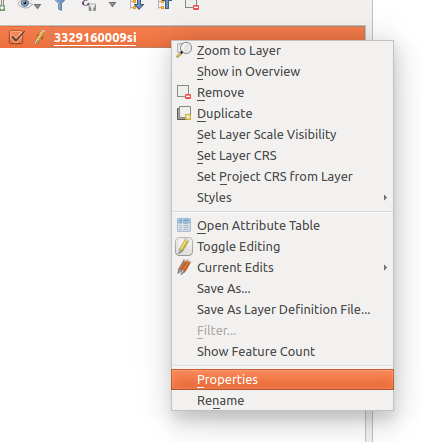
\includegraphics[scale=0.7]{./resources/038-layer-properties}
    \caption{Menu \textit{Layer Properties}}
    \label{fig:layerproperties}
  \end{figure}
  
  \item Pilih bagian \textit{Field}, setelah itu pada kolom \textit{Edit Widget} klik tombol \texttt{Text Edit} untuk kolom \texttt{d\_kd\_simbo} seperti gambar \ref{fig:layerpropertieswin}
  
  \begin{figure}[H]
    \centering
    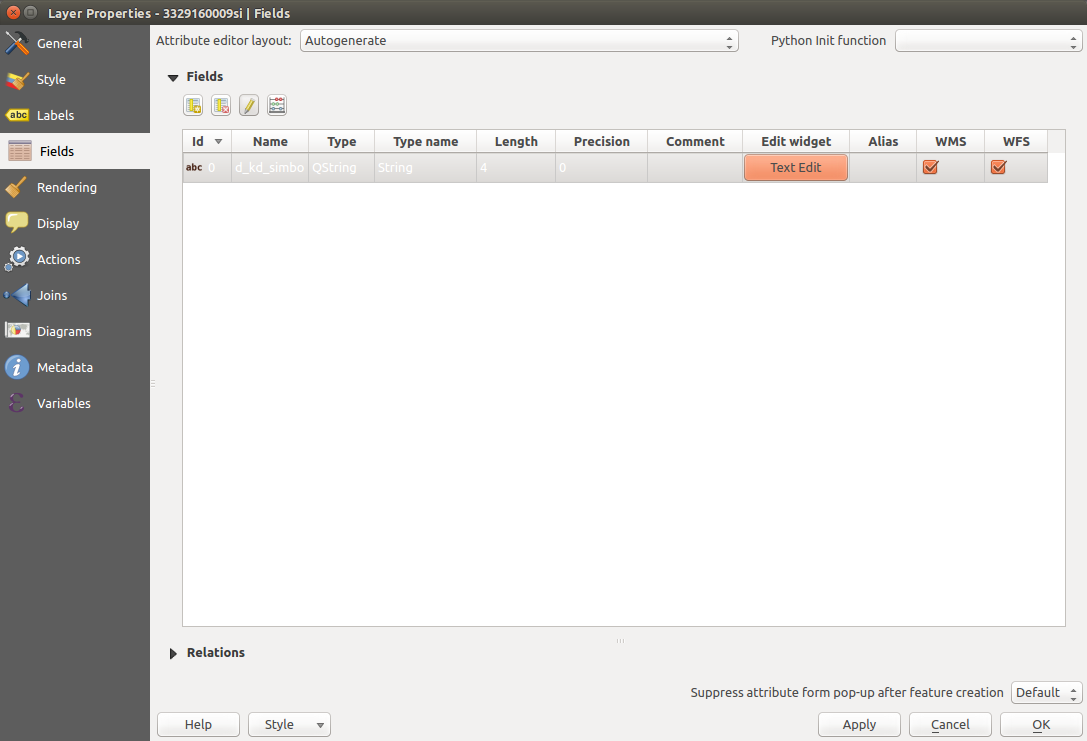
\includegraphics[width=1\textwidth]{./resources/039-jendela-layer-properties}
    \caption{Jendela \textit{Layer Properties}}
    \label{fig:layerpropertieswin}
  \end{figure}
  
  \item Pada menu \textit{Text Edit} pilih \textit{Value Map}, lalu isi nilai sesuai dengan ketentuan pengklasifikasian simbol dihalaman sebelumnya seperti pada gambar \ref{fig:simbolmapping}, klik \texttt{OK} pada kotak dialog \textit{edit attribute} dan klik \texttt{OK} pada menu \textit{field layer properties}.
  
  \begin{figure}[H]
    \centering
    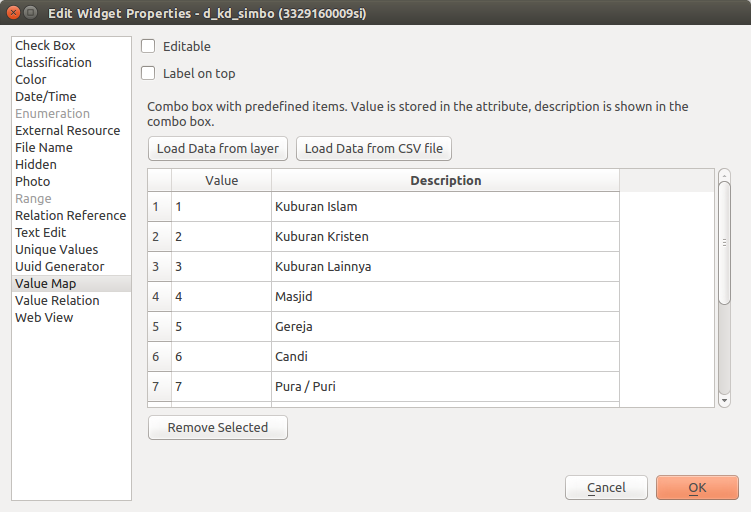
\includegraphics[width=1\textwidth]{./resources/040-mapping-simbol}
    \caption{\textit{Mapping} Simbol Untuk Mempermudah Pengisian}
    \label{fig:simbolmapping}
  \end{figure}
  
  \item Lakukan digitasi sesuai posisi yang diinginkan, dan pada akhir digitasi akan tampil kotak dialog seperti pada gambar \ref{fig:pilihanatribut} yang memungkinkan pengguna memilih isian untuk atribut tertentu.
  
  \begin{figure}[H]
    \centering
    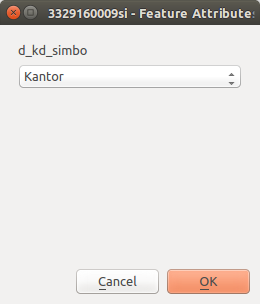
\includegraphics[width=1\textwidth]{./resources/041-pilihan-atribut}
    \caption{Pemilihan Isian untuk Atribut}
    \label{fig:pilihanatribut}
  \end{figure}
  
\end{enumerate}

\section{Edit Tabel Atribut}

\section{Memastikan CRS (\textit{Coordinate Reference System}) \textit{Settings}}

\section{Memulai Digitasi}

\section{\textit{Snapping Option}}

\backmatter%%%%%%%%%%%%%%%%%%%%%%%%%%%%%%%%%%%%%%%%%%%%%%%%%%%%%%%
\printindex

%%%%%%%%%%%%%%%%%%%%%%%%%%%%%%%%%%%%%%%%%%%%%%%%%%%%%%%%%%%%%%%%%%%%%%

\end{document}